\section{The mathematics: from phase difference to angle}
\label{sec:math}

This section is deliberately slow. Everything SPF does --- the beamformer
features fed to the networks, the symmetry constraints in training, the
particle filter's measurement model, and the dataset audit's forward model ---
is a consequence of one small piece of geometry, so it pays to derive it once,
carefully, with signs and conventions pinned down.

\subsection{Setup and conventions}
\label{sec:setup}

Two receive antennas $A_0$ and $A_1$ are separated by a baseline of length
$d$ (metres). Place the midpoint of the baseline at the origin, with the
baseline along the $x$-axis:
\[
A_0 = \left(+\tfrac{d}{2},\, 0\right), \qquad
A_1 = \left(-\tfrac{d}{2},\, 0\right).
\]
The \emph{boresight} (broadside) direction is the $+y$-axis, perpendicular to
the baseline. An emitter lies at range $R$ in direction $\theta$, where
$\theta$ is measured \emph{from boresight}, positive toward $+x$ (toward
$A_0$):
\[
E = (R\sin\theta,\; R\cos\theta).
\]
The emitter transmits a narrowband signal at carrier frequency $f$ with
wavelength $\lambda = c/f$ ($c$ the speed of light). At 2.412\,GHz,
$\lambda = 12.4$\,cm; at 5.766\,GHz, $\lambda = 5.2$\,cm; at 915\,MHz,
$\lambda = 32.8$\,cm.

\begin{figure}[ht]
\centering
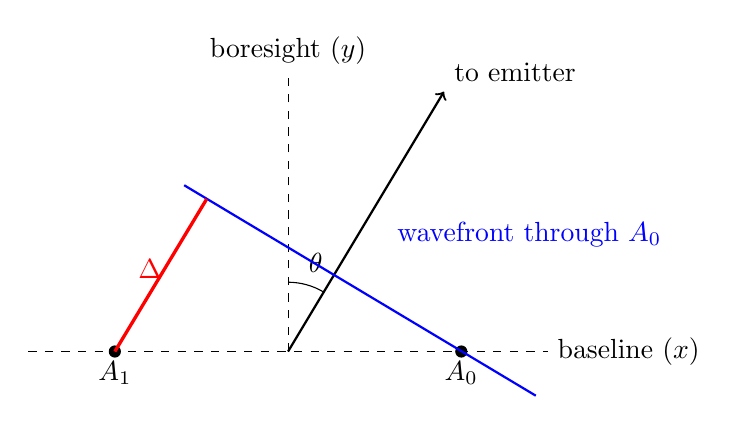
\begin{tikzpicture}[scale=1.1]
  % geometry precomputed for arrival direction u = (1.8,3.0)/|.| = (0.5145,0.8575),
  % i.e. theta = 31.0 deg east of boresight
  % antennas
  \fill (2,0) circle (2pt) node[below] {$A_0$};
  \fill (-2,0) circle (2pt) node[below] {$A_1$};
  \draw[dashed] (-3,0) -- (3,0) node[right] {baseline ($x$)};
  \draw[dashed] (0,0) -- (0,3.2) node[above] {boresight ($y$)};
  % arrival direction
  \draw[->,thick] (0,0) -- (1.8,3.0) node[above right] {to emitter};
  \draw (0,0.8) arc[start angle=90, end angle=59, radius=0.8];
  \node at (0.32,1.02) {$\theta$};
  % wavefront through A0: line through (2,0) perpendicular to u
  \draw[thick,blue] (2.86,-0.51) -- (-1.20,1.92);
  \node[blue, right] at (1.15,1.35) {wavefront through $A_0$};
  % extra path: A1 to its projection F = A1 + ((A0-A1).u) u = (-0.94,1.76)
  \draw[very thick,red] (-2,0) -- (-0.94,1.76);
  \node[red, left] at (-1.35,0.95) {$\Delta$};
\end{tikzpicture}
\caption{Far-field geometry. The wavefront (perpendicular to the arrival
direction) reaches $A_0$ first; $A_1$ waits for the wave to cover the extra
red path $\Delta = d\sin\theta$.}
\label{fig:geometry}
\end{figure}

\subsection{Step 1: the far-field assumption}
\label{sec:farfield}

Exactly, the two path lengths are $\lVert E - A_0\rVert$ and
$\lVert E - A_1\rVert$. Expanding $\lVert E - A_{0,1}\rVert$ in powers of
$d/R$:
\[
\lVert E - A_{0,1}\rVert
  = R \mp \tfrac{d}{2}\sin\theta
    + \frac{d^2\cos^2\theta}{8R} + O\!\left(\frac{d^3}{R^2}\right).
\]
The first-order term is the plane-wave (far-field) result; the quadratic term
is the near-field (wavefront curvature) correction. Its phase contribution is
$2\pi/\lambda \cdot d^2/(8R)$ at worst. Plugging in wall-array numbers
($d = 5$\,cm, $R = 0.9$\,m, $\lambda = 12.4$\,cm): the correction is
$\approx 0.018$\,rad --- negligible against measured phase noise, and it was
explicitly ruled out as a residual source in the audit. From here on we work
in the far field: incoming wavefronts are planes perpendicular to the arrival
direction.

\subsection{Step 2: path-length difference}
\label{sec:pathdiff}

Because the wavefronts are planes, the extra distance the wave must travel to
reach $A_1$ after passing $A_0$ is the projection of the baseline vector onto
the arrival direction (Figure~\ref{fig:geometry}). Write the unit vector
pointing \emph{from the array toward the emitter} as
$\hat u = (\sin\theta, \cos\theta)$. Then
\[
\Delta
 \;=\; (A_0 - A_1)\cdot \hat u
 \;=\; (d, 0)\cdot(\sin\theta, \cos\theta)
 \;=\; d\sin\theta .
\]
Sanity checks, worth internalizing:
\begin{itemize}
  \item \textbf{Broadside} ($\theta = 0$): $\Delta = 0$. Both antennas sit on
        the same wavefront; no delay.
  \item \textbf{Endfire} ($\theta = \pm 90^\circ$): $\Delta = \pm d$. The wave
        travels straight down the baseline; the delay is the full antenna
        separation.
  \item The dependence is on $\sin\theta$, not $\theta$: equal increments of
        angle near broadside change $\Delta$ much more than near endfire.
        This single fact drives the sensitivity analysis of
        Section~\ref{sec:sensitivity}.
\end{itemize}

\subsection{Step 3: from path difference to time delay to phase}
\label{sec:phase}

The wave covers the extra path $\Delta$ at speed $c$, so channel 1 receives a
copy of the signal delayed by
\[
\tau = \frac{\Delta}{c} = \frac{d\sin\theta}{c}.
\]
For a narrowband signal $s(t)\,e^{j2\pi f t}$ whose complex envelope $s(t)$
varies slowly over $\tau$ (always true here: $\tau \le d/c \sim 0.2$\,ns,
versus envelope timescales of $\ge$ tens of ns at our bandwidths), delay is
equivalent to a phase rotation of the carrier:
\[
x_0(t) = s(t)\, e^{j 2\pi f t}, \qquad
x_1(t) = s(t)\, e^{j 2\pi f (t - \tau)}
       = x_0(t)\, e^{-j 2\pi f \tau}.
\]
Define the \textbf{measured phase difference} as the phase of channel 1
relative to channel 0:
\[
\boxed{\;
\varphi \;=\; \arg\!\big(x_1 x_0^{*}\big)
        \;=\; -\,2\pi f \tau
        \;=\; -\,2\pi \frac{d \sin\theta}{\lambda}
        \;=\; -\,2\pi\,\dlam\,\sin\theta .
\;}
\]
This is the entire physical content of a two-element array: \emph{one
sinusoid-of-angle, scaled by the spacing in wavelengths}. The sign is a
convention (it flips if you swap antenna labels, measure $\theta$ from the
other side, or conjugate the wrong channel); SPF fixes it by the definition
above, and the audit's forward model uses exactly this expression with
$\theta$ replaced by $\theta - \theta_{\mathrm{mount}}$ (the array's own
orientation).

Worked micro-examples with $\dlam = \tfrac12$ (the classic half-wavelength
array, $\varphi = -\pi\sin\theta$):
\begin{center}
\begin{tabular}{rrr}
\toprule
$\theta$ & $\sin\theta$ & $\varphi$ \\
\midrule
$0^\circ$   & $0$     & $0$ \\
$+30^\circ$ & $0.5$   & $-\pi/2 \approx -1.571$ \\
$+90^\circ$ & $1$     & $-\pi$ \\
$-30^\circ$ & $-0.5$  & $+\pi/2$ \\
$-90^\circ$ & $-1$    & $+\pi$ \\
\bottomrule
\end{tabular}
\end{center}
Note $\theta = +90^\circ$ and $-90^\circ$ give $-\pi$ and $+\pi$ --- the same
angle modulo $2\pi$. Even the ideal half-wavelength array is only
\emph{just barely} unambiguous.

\subsection{Step 4: estimating $\varphi$ from IQ samples}
\label{sec:estimation}

With sampled complex baseband $x_0[n], x_1[n]$, form the per-sample product
$z[n] = x_1[n]\, x_0^{*}[n]$. Its phase is $\varphi$ plus noise; its magnitude
is the product of channel amplitudes. The maximum-likelihood-style estimate
over a window $W$ is the phase of the \emph{coherent sum}:
\[
\hat\varphi \;=\; \arg \sum_{n \in W} x_1[n]\, x_0^{*}[n].
\]
Three properties matter in practice:
\begin{enumerate}
  \item \textbf{It is a circular mean.} Averaging $z[n]$ in the complex plane
        before taking $\arg$ handles phase wrapping correctly; averaging raw
        phases does not ($+179^\circ$ and $-179^\circ$ average to $0^\circ$
        instead of $180^\circ$).
  \item \textbf{It is amplitude-weighted.} Strong samples dominate the sum.
        Usually good (they have better SNR), but under fast-attack AGC the
        amplitude is a moving target --- gain steps within a window distort
        the weighting, and gain-index changes can flip channel polarity
        (a $\pi$ error on the affected samples).
  \item \textbf{Windowing trades variance for time resolution.} SPF computes
        $\hat\varphi$ (and a full beamformer, below) over many short windows
        per capture snapshot rather than one long one, retaining the
        distributional shape --- which the networks consume and the audit
        summarizes with circular statistics.
\end{enumerate}

The same window statistic generalizes to the \textbf{beamformer}: for each
candidate angle $\theta_k$ on a grid (SPF uses 65 bins), the steering weight
$e^{+j2\pi \dlam \sin\theta_k}$ is applied and the coherently combined power
recorded. For two elements this is mathematically just
$\big|1 + e^{j(\varphi + 2\pi\dlam\sin\theta_k)}\big|^2$ --- a raised cosine
in $\sin\theta_k$ peaked wherever $\varphi$ is explained --- so the
beamformer output is an \emph{ambiguity-faithful likelihood over angle}, not
a decision. That is exactly why it is the right network input: it encodes
what the physics knows, including every alias peak, and lets the model (and
the filter) do the disambiguation.

\subsection{Step 5: inverting phase to angle --- and the two ambiguities}
\label{sec:ambiguity}

Naively inverting the boxed equation:
\[
\hat\theta \;=\; \arcsin\!\left( -\,\frac{\hat\varphi}{2\pi}\,
                                 \frac{\lambda}{d} \right).
\]
Two distinct ambiguities interfere with this inversion.

\paragraph{Ambiguity 1: front--back (mirror) symmetry.}
$\Delta = d\sin\theta$ depends only on the projection of the arrival
direction onto the baseline. A source at $\theta$ and its mirror image at
$\pi - \theta$ (same $x$-component, opposite $y$) produce \emph{identical}
$\Delta$, hence identical $\varphi$, for every spacing and wavelength:
\[
\sin(\pi - \theta) = \sin\theta .
\]
A linear two-element array is physically incapable of telling front from
back. SPF therefore works in the folded half-space
$\theta \in [-\pi/2, +\pi/2]$ (``reduced theta'') at the single-radio level,
and resolves the mirror only by fusion: two arrays with different mount
orientations on one platform, or one array observed along a trajectory,
disagree about the mirror image but agree about the true source.

\paragraph{Ambiguity 2: phase wrapping / grating lobes.}
The measurable phase is only known modulo $2\pi$:
$\hat\varphi \in (-\pi, \pi]$ (SPF's $\pinorm$). The true geometric phase
$-2\pi\dlam\sin\theta$ ranges over $[-2\pi\dlam,\, +2\pi\dlam]$, an interval
of total width $4\pi\dlam$. Uniqueness of the inversion requires that width
to fit inside one $2\pi$ turn:
\[
4\pi\,\dlam \le 2\pi
\quad\Longleftrightarrow\quad
\boxed{\; d \le \frac{\lambda}{2} \;}
\]
--- the classical half-wavelength criterion, the spatial twin of Nyquist
sampling. When $d > \lambda/2$, all angles
\[
\theta_k = \arcsin\!\left( -\frac{\lambda}{d}
           \left( \frac{\hat\varphi}{2\pi} + k \right) \right),
\qquad k \in \mathbb{Z},\;
\left| \frac{\hat\varphi}{2\pi} + k \right| \le \dlam,
\]
are exactly consistent with the measurement --- the grating lobes. The number
of consistent angles is roughly $\lceil 2\dlam \rceil$ per half-space.

SPF's fleet spans $\dlam \approx 0.21$ to $1.55$. At $\dlam = 1.27$ (a common
5.8\,GHz configuration) a single snapshot admits $\sim$3 candidate bearings
per half-space, times the front--back mirror: up to six angles indistinguishable
from one measurement. This is \emph{by design}: larger $\dlam$ buys angular
resolution (next subsection) at the price of ambiguity, and the ambiguity is
handed to the learned models and the particle filter, which see many
snapshots, two radios, and motion.

\subsection{Step 6: sensitivity, resolution, and where the information lives}
\label{sec:sensitivity}

Differentiate the forward model:
\[
\frac{d\varphi}{d\theta} = -\,2\pi\,\dlam\,\cos\theta .
\]
A phase-noise floor $\sigma_\varphi$ therefore maps to bearing noise
\[
\sigma_\theta \;\approx\; \frac{\sigma_\varphi}{2\pi\,\dlam\,|\cos\theta|}.
\]
Consequences:
\begin{itemize}
  \item \textbf{Broadside is the sweet spot}; at endfire
        ($\theta \to \pm 90^\circ$) the derivative vanishes and bearing
        information disappears entirely --- no estimator can fix this.
  \item \textbf{Wider spacing is better, linearly}, wherever the alias
        candidates can be resolved by other means. Doubling $\dlam$ halves
        $\sigma_\theta$. This is the quantitative argument for collecting
        data at $\dlam$ well beyond $1/2$ and treating disambiguation as a
        separate, solvable problem.
  \item With measured wall-array phase noise $\sigma_\varphi \sim 0.5$\,rad
        (corrected residual, good datasets) and $\dlam = 0.5$:
        $\sigma_\theta \approx 0.16$\,rad $\approx 9^\circ$ per window at
        broadside --- and windows arrive by the hundreds per second, so the
        per-snapshot posterior tightens fast if systematics don't bias it.
\end{itemize}

\subsection{Step 7: the real world --- a three-parameter systematic model}
\label{sec:systematics}

Real rigs deviate from the boxed model in low-dimensional, physically
interpretable ways. The audit fits, per dataset and per channel pair, using
ground-truth bearing $\theta_{\mathrm{gt}}$:
\[
\varphi \;\approx\; c \;+\; g \cdot
   \Big(-2\pi\,\dlam\Big)\,
   \sin\!\big(\theta_{\mathrm{gt}} - \Delta\theta\big),
\]
with exactly three parameters:
\begin{description}
  \item[$c$ (phase offset):] a constant inter-channel phase --- LO
        distribution, cable-length mismatch, front-end group delay. Harmless
        to a learned model (it is per-rig constant) but fatal to naive
        inversion.
  \item[$g$ (gain of the sine, equivalently effective$/$configured spacing):]
        $g \ne 1$ means the array behaves as if its spacing were
        $g\,d$. Causes: mislabeled physical spacing (documented and later
        hand-fixed for a batch of rover captures: 43\,mm labels on a 47\,mm
        array), antenna coupling and connector geometry (the wall fleet shows
        an effective-spacing floor of $\approx$6--7\,cm at 2.4\,GHz
        regardless of smaller configured values), frequency-dependent
        electrical length. The audit's receiver-agreement correlation
        ($\rho \approx 0.64$ between the two independent receivers of the
        same session) shows $g$ is a real physical property, not fit noise.
  \item[$\Delta\theta$ (angular offset):] mount rotation relative to the
        platform frame, or --- on rovers --- compass bias. Era-dependent on
        rovers (a compass recalibration event visibly moved the fleet-wide
        bias from $-0.15$\,rad to $+0.04$\,rad).
\end{description}
The decomposition matters because the three parameters are \emph{corrections}
(deterministic, learnable, even fixable in metadata), while what remains
after the fit --- the corrected residual spread --- is genuine measurement
noise. The audit treats them differently: systematic terms feed
``label-correction'' candidate lists; residual spread feeds quality gates.

\subsection{Step 8: quantifying the leftover noise --- circular statistics}
\label{sec:circstats}

Residuals $\delta\varphi = \pinorm(\hat\varphi - \varphi_{\mathrm{model}})$
live on the circle, so ordinary standard deviation is wrong near the wrap.
With unit phasors $e^{j\delta\varphi_i}$ and resultant length
\[
\bar R = \Big| \tfrac{1}{N}\sum_{i=1}^{N} e^{j\delta\varphi_i} \Big|
\in [0, 1],
\]
the circular standard deviation is
\[
\sigma_{\mathrm{circ}} = \sqrt{-2\ln \bar R}.
\]
Interpretation anchors: $\sigma_{\mathrm{circ}} \approx$ the ordinary
$\sigma$ for concentrated data ($\lesssim 0.5$); a uniform (information-free)
phase distribution gives $\bar R \to 0$ and a finite-$N$ floor of
$\sigma_{\mathrm{circ}} \approx 2.1$ at $N = 50$ rising to $\approx 3.0$ at
$N = 5000$; and mixtures are nonlinear --- 30\% uniform junk contaminating an
otherwise clean channel already pushes $\sigma_{\mathrm{circ}}$ to
$\approx 0.9$. Heavy tails from AGC gain steps and LNA-bypass polarity flips
($\pi$ jumps) inflate it further. These anchors calibrate every quality gate
in the audit.

\subsection{Summary of the chain}

\[
\theta
\;\xrightarrow{\;\text{geometry}\;}
\Delta = d\sin\theta
\;\xrightarrow{\;\tau = \Delta/c\;}
\varphi = -2\pi\dlam\sin\theta
\;\xrightarrow{\;\text{rig}\;}
c + g(\cdot)\;\text{at}\;\theta - \Delta\theta
\;\xrightarrow{\;\text{noise}\;}
\hat\varphi
\]
Reading the chain left to right generates predictions (the beamformer, the
audit's forward model); reading it right to left --- through wrapping,
aliasing, mirrors, systematics, and noise --- is the estimation problem the
learned models and filters solve.
